\documentclass{report}
\usepackage[french]{babel}

\usepackage[letterpaper,top=2cm,bottom=2cm,left=3cm,right=3cm,marginparwidth=1.75cm]{geometry}

% Useful packages
\usepackage{algorithme}
\usepackage{comment}
\usepackage[T1]{fontenc}
\usepackage{fullpage}
\usepackage{color}
\usepackage{listings}
\usepackage{xcolor}
\usepackage{pdfpages}
\usepackage{graphicx}
\usepackage{hyperref} 
\usepackage{tabularx}
\usepackage{parskip}

\setlength{\parindent}{20pt}


\hypersetup{ 
    colorlinks,
    citecolor=black,
    filecolor=black,
    linkcolor=black,
    urlcolor=black
}
\lstset{language=C,
	literate=
  {²}{{\textsuperscript{2}}}1
  {⁴}{{\textsuperscript{4}}}1
  {⁶}{{\textsuperscript{6}}}1
  {⁸}{{\textsuperscript{8}}}1
  {€}{{\euro{}}}1
  {é}{{\'e}}1
  {è}{{\`{e}}}1
  {ê}{{\^{e}}}1
  {ë}{{\¨{e}}}1
  {É}{{\'{E}}}1
  {Ê}{{\^{E}}}1
  {û}{{\^{u}}}1
  {ù}{{\`{u}}}1
  {â}{{\^{a}}}1
  {à}{{\`{a}}}1
  {á}{{\'{a}}}1
  {ã}{{\~{a}}}1
  {Á}{{\'{A}}}1
  {Â}{{\^{A}}}1
  {Ã}{{\~{A}}}1
  {ç}{{\c{c}}}1
  {Ç}{{\c{C}}}1
  {õ}{{\~{o}}}1
  {ó}{{\'{o}}}1
  {ô}{{\^{o}}}1
  {Õ}{{\~{O}}}1
  {Ó}{{\'{O}}}1
  {Ô}{{\^{O}}}1
  {î}{{\^{i}}}1
  {Î}{{\^{I}}}1
  {í}{{\'{i}}}1
  {Í}{{\~{Í}}}1,
	breaklines,
	frame=tb, % draw a frame at the top and bottom of the code block
    tabsize=4, % tab space width
    showstringspaces=false, % don't mark spaces in strings
    numbers=left, % display line numbers on the left
    commentstyle=\color{violet}, % comment color
    keywordstyle=\color{blue}, % keyword color
    stringstyle=\color{red} % string color
}
\title{Projet Othello - Rapport}
\author{Benchekroun Yasmine, Charles Lucas, Essakhi Jihane, Foyer Laurent}

\begin{document}
  
\maketitle

\chapter{Introduction}

    L'Othello, une variante du Reversi, est un jeu de stratégie se jouant à deux joueurs sur un plateau de 8x8 cases : l'objectif de ce jeu est de placer des pions tour par tour de manière à contrôler le plus de cases possible sur le plateau. \par
    
    Le projet détaillé dans ce rapport, réalisé au cours de 10 semaines du 25 octobre 2022 au 3 janvier 2023, consiste à la programmation d'un jeu d'Othello permettant de jouer contre un ordinateur via le développement d'une IA. Celui-ci doit permettre au joueur de choisir sa couleur (noir ou blanc) ainsi que la difficulté de l'IA (la profondeur, qui le plus élevée elle est rend en principe l'IA meilleure au jeu). De plus, le jeu doit pouvoir participer à un mode "tournoi" dans lequel il pourra affronter l'IA d'un autre programme en communiquant via un protocole prédéterminé. \par

    Développé en C, celui-ci a dû être conçu suivant l'ensemble des étapes du cycle en V : analyse, conception préliminaire, conception détaillée, et développement, ainsi que la réalisation de leurs tests associés. Ce rapport détaille dans son ensemble les fonctions et algorithmes utilisées dans la réalisation du jeu d'Othello.

\chapter{Analyse descendante}
    \vspace*{2cm}
    \noindent
    \makebox[\textwidth]{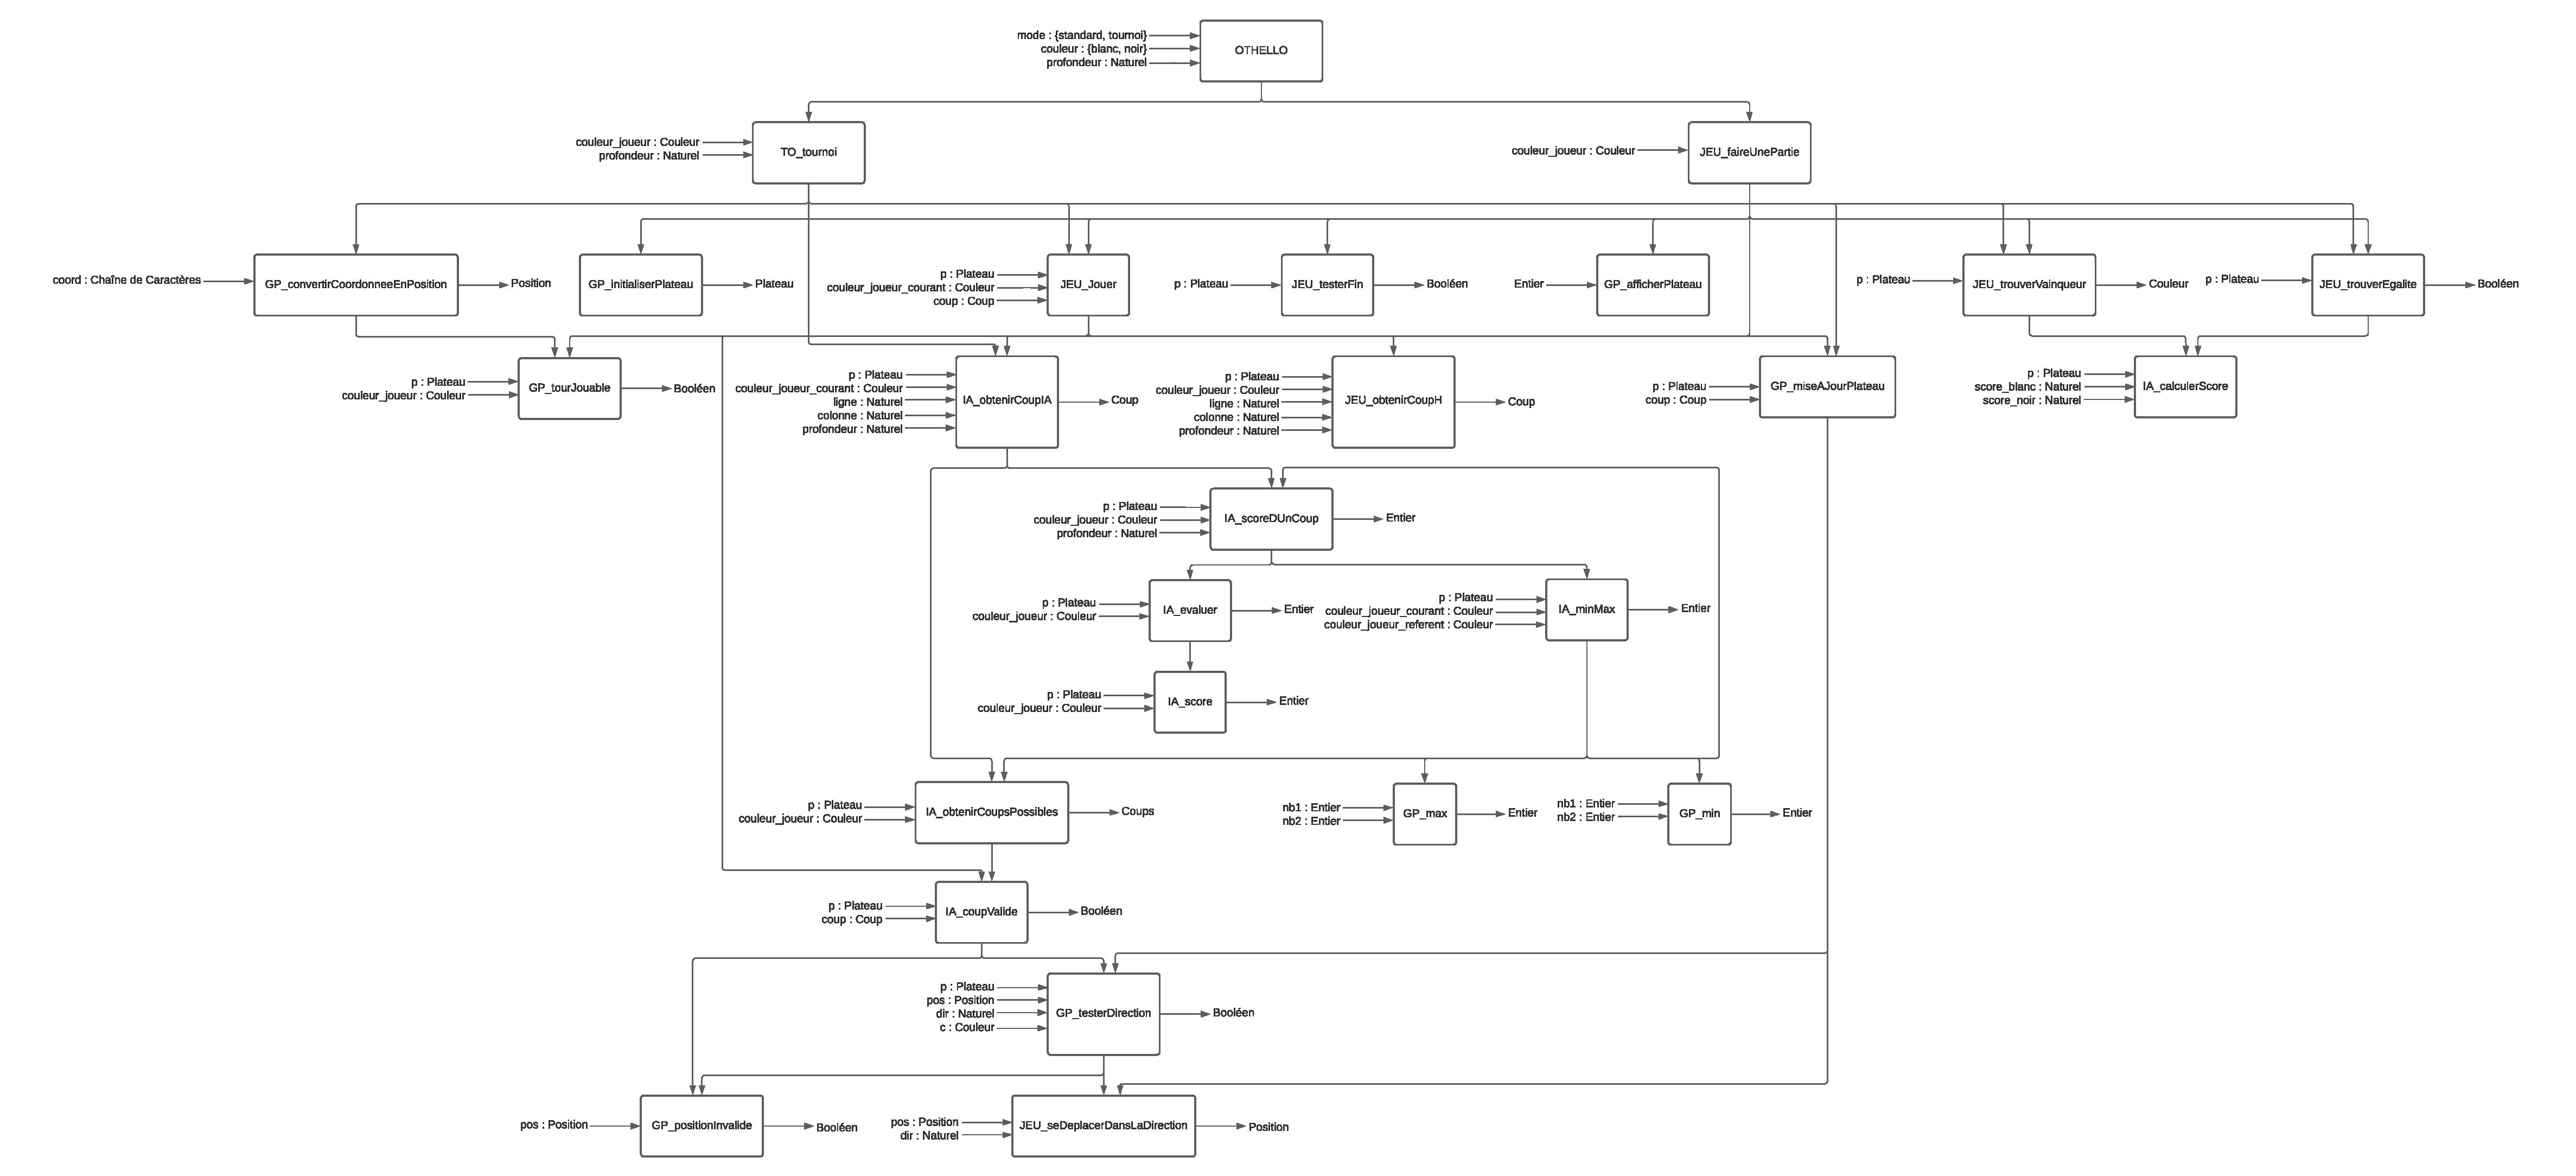
\includegraphics[scale=0.26, angle=0]{Analyse_descendante.pdf}}%
    \vspace*{\fill}
\chapter{Analyses}
\section{Présentation des TAD}

    \subsection{TAD Couleur}
    \begin{tad}
    \tadNom{Couleur}
    \tadDependances{\booleen}
    \begin{tadOperations}{couleur}
    \tadOperation{couleur}{\booleen}{\tadUnParam{Couleur}}
    \tadOperation{couleurOpposée}{\tadUnParam{Couleur}}{\tadUnParam{Couleur}}
    \tadOperation{couleurIdentiques}{\tadDeuxParams{Couleur}{Couleur}}{\tadUnParam{\booleen}}
    \end{tadOperations}
    \begin{tadAxiomes}
      \tadAxiome{$couleur(1) = BLANC$}
      \tadAxiome{$couleur(0) = NOIR$}
    \end{tadAxiomes}
    \end{tad} 
    
    \subsection{TAD Pion}
    \begin{tad}
    \tadNom{Pion}
    \tadDependances{Position, Couleur}
    \begin{tadOperations}{pion}
      \tadOperation{pion}{\tadDeuxParams{Couleur}{Position}}{\tadUnParam{Pion}}
      \tadOperation{obtenirPosition}{\tadUnParam{Pion}}{\tadUnParam{Position}}
      \tadOperation{obtenirCouleur}{\tadUnParam{Pion}}{\tadUnParam{Couleur}}
      \tadOperation{changerCouleur}{\tadUnParam{Pion}}{\tadUnParam{Pion}}
      \tadOperation{estPlace}{\tadUnParam{Pion}}{\tadUnParam{\booleen}}
      \tadOperation{fixerCouleur}{\tadDeuxParams{Pion}{Couleur}}{\tadUnParam{Pion}}
      
    \end{tadOperations}
    \begin{tadAxiomes}
      \tadAxiome{si $obtenirCouleur(p1) = NOIR$ alors $obtenirCouleur(changerCouleur(p1)) = BLANC$}
      \tadAxiome{si $obtenirCouleur(p1) = BLANC$  alors $obtenirCouleur(changerCouleur(p1)) = NOIR$}
    \end{tadAxiomes}
    \end{tad}  
    
    \subsection{TAD Position}
    \begin{tad}
    \tadNom{Position}
    \tadDependances{Naturel Non Nul, Booléen, Plateau}
    \begin{tadOperations}{position}
      \tadOperation{position}{\tadDeuxParams{$[1..8]$}{$[1..8]$}}{\tadUnParam{Position}}
      \tadOperation{obtenirLigne}{\tadUnParam{Position}}{\tadUnParam{$[1..8]$}}
      \tadOperation{obtenirColonne}{\tadUnParam{Position}}{\tadUnParam{$[1..8]$}}
      
    \end{tadOperations}
    \begin{tadAxiomes}
      \tadAxiome{$obtenirLigne(position(x,y)) = x$}
      \tadAxiome{$obtenirColonne(position(x,y)) = y$}
    \end{tadAxiomes}
    \end{tad}  
    
    \subsection{TAD Plateau}
    \begin{tad}
    \tadNom{Plateau}
    \tadDependances{Naturel Non Nul, Couleur, Naturel , Pion}
    \begin{tadOperations}{plateau}
      \tadOperation{plateau}{}{\tadUnParam{Plateau}}
      \tadOperation{obtenirHauteur}{\tadUnParam{Plateau}}{\tadUnParam{\naturel}}
      \tadOperation{obtenirLargeur}{\tadUnParam{Plateau}}{\tadUnParam{\naturel}}
      \tadOperation{testerFin}{\tadUnParam{Plateau}}{\tadUnParam{\booleen}}
      \tadOperation{estplein}{\tadUnParam{Plateau}}{\tadUnParam{\booleen}}
      \tadOperation{obtenirPion}{\tadDeuxParams{Plateau}{Position}}{\tadUnParam{Pion}}
      \tadOperation{nbPionsDUneCouleur}{\tadDeuxParams{Plateau}{Couleur}}{\tadUnParam{\naturel}}
      \tadOperation{placerPion}{\tadDeuxParams{Plateau}{Pion}}{\tadUnParam{Plateau}}
      \tadOperation{memePlateau}{\tadDeuxParams{Plateau}{Plateau}}{\tadUnParam{Plateau}}
      \tadOperation{copier}{\tadUnParam{Plateau}}{\tadUnParam{Plateau}}
      \tadOperation{effacer}{\tadUnParam{Plateau}}{\tadUnParam{Plateau}}
      \tadOperation{mettreÀJourPlateau}{\tadUnParam{Plateau}}{\tadUnParam{Plateau}}
      
    \end{tadOperations}
    \end{tad}  

    \subsection{TAD Coup}
    \begin{tad}
    \tadNom{Coup}
    \tadDependances{Pion, Plateau}
    \begin{tadOperations}{coup}
      \tadOperation{coup}{\tadUnParam{Pion}}{\tadUnParam{Coup}}
      \tadOperation{jouerCoup}{\tadDeuxParams{Plateau}{Coup}}{\tadUnParam{Plateau}}
      \tadOperation{obtenirPion}{\tadUnParam{coup}}{\tadUnParam{Pion}}
    
      
    \end{tadOperations}
    \end{tad}
    
        
        
    \subsection{TAD Coups}
    \begin{tad}
    \tadNom{Coups}
    \tadDependances{Coup, Booléen, Naturel , ListeCoups}
    \begin{tadOperations}{coups}
      \tadOperation{coups}{}{\tadUnParam{Coups}}
      \tadOperation{ajouterCoup}{\tadDeuxParams{coups}{Coup}}{\tadUnParam{Coups}}
      \tadOperation{estVide}{\tadUnParam{Coups}}{\tadUnParam{\booleen}}
      \tadOperation{nbCoups}{\tadUnParam{Coups}}{\tadUnParam{\naturel}}
      \tadOperation{obtenirIEmeCoup}{\tadDeuxParams{Coups}{\naturel}}{\tadUnParam{Coup}}
    \end{tadOperations}

    
    \begin{tadAxiomes}
      \tadAxiome{$estVide(coups())$}
      \tadAxiome{non $estVide(ajouterCoup(cps,c))$}
    \end{tadAxiomes}
    \end{tad}
    \section{Conception préliminaire}
        \subsection{ Signatures des fonction / procédures utilisées }
        \begin{itemize}
         \item {\tt Procédure TO\_tournoi( E couleur : Couleur , Profondeur: \naturel )}
         \item{\tt Procédure JEU\_faireUnePartie( E couleur\_Joueur : Couleur)}
         \item{ \tt fonction GP\_convertirCoordonneeEnPosition ( coord : Chaine de caractères) : Position}
         \item{\tt fonction GP\_intialiserPlateau() : Plateau }
         \item{\tt procédure JEU\_Jouer (E couleur\_joueur\_courant : Couleur  , coup : Coup , E/S p : Plateau) }
         \item{\tt fonction JEU\_testerFin(p:Plateau):\booleen }
         \item{\tt  fonction GP\_afficherPlateau(P : plateau)}
         \item{\tt  fonction JEU\_troouverVainqueur(p : Plateau):Couleur}
         \item{\tt fonction JEU\_trouverEgalite(p : Plateau): \booleen}
         \item{\tt  procédure IA\_calculerScore( E p : Plateau , E/S score\_blanc , score\_noir: Naturel )}
         \item{ \tt fonction GP\_tourJouable( p : Plateau , couleur\_joueur : Couleur) : \booleen}
         \item{\tt  fonction IA\_obtenirCoupIA (p:Plateau , couleur\_joueur\_courant : Couleur , ligne : \naturel, colonne : \naturel , profondeur : \naturel ):Coup}
         \item{\tt fonction IA\_scoreDUnCoup (p:Plateau , couleur\_joueur : Couleur , profondeur : \naturel}:\naturel
          
           \item {\tt fonction IA\_evaluer(p : Plateau, couleur\_joueur :Couleur) : Entier}
           \item {\tt fonction IA\_score(p : Plateau, couleur\_joueur :Couleur) : Entier}
           \item {\tt fonction minMax(p : Plateau, couleur\_joueur\_courant , couleur\_joueur\_referent : Couleur) : Entier}
           
         \item{\tt fonction IA\_obtenirCoupsPossibles(p : Plateau , couleur\_joueur : Couleur):Coups}
         \item{\tt fonction GP\_max(nb1 , nb2 : Entier):Entier}
         \item{\tt fonction GP\_min(nb1 , nb2 : Entier):Entier}
         \item{\tt fonction IA\_coupValide(p : Plateau , coup : Coup):\booleen}
         \item{\tt  fonction JEU\_obtenirCoupH (p : Plateau , couleur\_Joueur : Couleur , ligne : \naturel , colonne : \naturel , profondeur : \naturel): Coup}
         \item{\tt Procédure GP\_MiseAJourPlateau( E coup : Coup , E/S p: Plateau)}
          
         \item{\tt fonction GP\_testerDirection(p : Plateau pos : Position dir : Naturel c : Couleur)\booleen}
         \item{\tt fonction GP\_positionInvalide(pos : Position):\booleen}
         \item{\tt fonction JEU\_seDeplacerDansLaDirection(pos : Position , dir : \naturel): Position}
       
        
        \end{itemize}
    \chapter {Conception détaillée}
    
        \section{Conception détaillée des TAD}
         \begin{itemize}
             \item TAD Couleur = Structure 
             \begin{itemize}
             \item couleur = \booleen
             \end{itemize}
             \item TAD Pion = Structure
             \begin{itemize}
                 \item position = Position
                 \item couleur = Couleur
                 \item estPlacé = \booleen
             \end{itemize}
             \item TAD Position = Structure
             \begin{itemize}
                 \item ligne = 1..8
                 \item colonne = 1..8
             \end{itemize}
             \item TAD Plateau = Structure
             \begin{itemize}
                 \item lesPions = Tableau[8][8] de Pions
                 \item estPlein = Booléen
                 \item nbPionsPlaces = 1..64
             \end{itemize}
             \item Coup = Pion
             \item Coups = Liste [1..MAX] de Coup
         \end{itemize}
         
         \section{Conception détaillée des fonctions et procédures}
         

            \subsubsection{Fonctions et procédures qui permettent de jouer une partie}
            \subsubsection{ Procédure JEU\_faireUnePartie}
            
            \begin{algorithme}
\procedure{JEU\_faireUnePartie}{\paramEntree couleur\_chosie : Couleur}{p : Plateau , profondeur : \naturel , vainqueur ; Couleur , egalite: \booleen , nb\_tour : \naturel , couleur\_joueur\_humain , couleur\_joueur\_courant : Couleur , ligne : \naturel , colonne : \caractere , str : Tableau[1..2] de \caractere }{\affecter{nb\_tour}{0}
            \affecter{couleur\_joueur\_humain}{couleur\_choisie}
            \affecter{couleur\_joueur\_courant}{couleur\_joueur\_humain}
            \affecter{p}{ GP\_initialiserPlateau()}
            \instruction{IHM\_gras("Vous commencez !")}
    \instruction{IHM\_gras("Avec quelle profondeur voulez vous que l'IA joue ?")}
    \lire{profondeur}
    \tantque{non JEU\_testerFin(p)}{\affecter{nb\_tour}{nb\_tour + 1}
    \instruction{IHM\_separateur()}
    \instruction{GP\_afficherPlateau(p)}
    \sialorssinon{couleursIdentiques(couleur\_joueur\_courant,couleur\_joueur\_humain)}{ 
    \instruction{IHM\_gras("À vous de jouer !\")}
    {\repeter{
    \instruction{IHM\_gras("Quel coup voulez-vous jouer ? Entrez une lettre suivie d'un chiffre :  ")} 
    \lire{str}
    \affecter{ligne}{str[1]}
    \affecter{colonne}{str[0]}
      \sialors{non IA\_coupValide(p,coup(pion(couleur\_joueur\_humain,position(ligne,colonne))))}{\instruction{IHM\_gras("Coup non valide, réessayez !")}}
      }
    {\instruction{IA\_coupValide(p,coup(TADPion\_pion(couleur\_joueur\_humain ,Position\_position(ligne,colonne)))))}}}
    \instruction{JEU\_jouer(p,couleur\_joueur\_courant,JEU\_obtenirCoupH,ligne,colonne,3)}
}{
\instruction{JEU\_jouer(p,couleur\_joueur\_courant, IA\_obtenirCoupIA,0,0,profondeur)}}
\affecter{couleur\_joueur\_courant}{couleurOpposee(couleur\_joueur\_courant)}
            }\instruction{IHM\_gras("La partie est terminée ! ")}
            \affecter{egalite}{JEU\_trouverEgalite(p)}
              \sialorssinon{ non egalite}{
              \affecter{vainqueur
              }{JEU\_trouverVainqueur(p)}
              \ecrire{" Le vainqueur est la couleur",obtenircouleur(vainqueur))}}
              {\instruction{GP\_afficherPlateau(p)}
              \ecrire{"Pas de vainqueur !"}}
}
\end{algorithme}
  \bigskip 
         
            \subsubsection{ Procédure JEU\_jouer}
            \begin{algorithme}
\procedure{JEU\_jouer}{\paramEntreeSortie{p : Plateau}
            \paramEntree{ couleur\_joueur\_courant : Couleur}}{coup\_joue : Coup }{
            \sialorssinon{GP\_tourJouable(p, couleur\_joueur\_courant)}{
            \affecter{coup\_joue}{obtenirCoup(p,couleur\_joueur\_courant,3)
            \instruction{ JEU\_jouerCoup(p,coup\_joue)}
            \instruction{GP\_miseAJourPlateau(p,coup\_joue)}
            }}{\ecrire{" Tour sauté !"}}}
\end{algorithme}
  \bigskip 
            
             \subsubsection{Fonction JEU\_obtenirCoupH}
               \begin{algorithme}
 \fonction{JEU\_obtenirCoupH}{p : plateau , couleur\_joueur : Couleur , ligne : \naturel , colonne : \caractere , profondeur : \naturel}{Coup}{coup : Coup }
             { 
             \affecter{coup}{coup(pion(couleur\_joueur, position(ligne,colonne)))}
             \retourner{coup}
             }
 \end{algorithme}
  \bigskip 
            
             \subsubsection{Fonction seDeplacerDansLaDirection}
               \begin{algorithme}
 \procedure{seDeplacerDansLaDirection}{\paramEntreeSortie{pos : Position}, \paramEntree{dir : \naturel}}{dirLigne , dirColonne : Tableau [1..8] d'Entier}{
             \affecter{dirLigne}{[-1,-1,0,1,1,1,0,-1]}
             \affecter{dirLigne}{[{0,1,1,1,0,-1,-1,-1}]}
             \retourner{Position\_position(Position\_obtenirLigne(pos) + dirLigne[dir] , Position\_obtenirColonne(pos) + dirColonne[dir])}
             }
  \end{algorithme}
  \bigskip 
            
             \subsubsection{JEU\_trouverVainqueur}
              \begin{algorithme}
\fonction{JEU\_trouverVainqueur}{p1 : Plateau}{Couleur}{Taille : \naturel , egalite : \naturel , \naturel egalite , vainqueur : Couleur , score\_blanc, score\_noir : \naturel}{\affecter{TAILLE}{8}\affecter{egalite}{(score\_blanc = score\_noir)}{\sialorssinon{egalite}{\affecter{vainqueur}{couleur(Vrai)}}{\sialorssinon{score\_blanc $>$
               score\_noir}{\affecter{vainqueur }{couleur(vrai)}}{\affecter{vainqueur}{couleur(Faux)}}}} \retourner{vainqueur}}
               \end{algorithme}
  \bigskip 

               \subsubsection{fonction JEU\_trouverEgalite}
                \begin{algorithme}
 \fonction{JEU\_trouverEgalite}{ p1: Plateau}{\booleen}{score\_blanc , score\_noir : \naturel , egalite : \booleen}{ \instruction{JEU\_calculerScore(pl,score\_blanc,score\_noir)}
      \affecter{egalite}{(score\_blanc = score\_noir)}
      \retourner{egalite}
      }
 \end{algorithme}
  \bigskip  
            
               \subsubsection{JEU\_testerFin}
                \begin{algorithme}
\fonction{JEU\_testerFin}{p : Plateau }{\booleen}{}{
             \sialors{(Plateau\_estPlein(p)) et (non GP\_tourJouable(p, couleur(1)))}{\retourner{1))}
             \sialorssinon{non GP\_tourJouable(p, couleur(0))}{\retourner{1}}{\retourner{0}}
             }}
\end{algorithme}
  \bigskip 
             
             \subsubsection{Procédure JEU\_calculerScore}
              \begin{algorithme}
\procedure{JEU\_calculerScore}{\paramEntree{p1 : Plateau} \paramEntreeSortie{score\_blanc : \naturel , score\_noir : \naturel }}{ TAILLE : \naturel , blanc , noir : Couleur , position : Position , pion : Pion}{\affecter{TAILLE}{8}
             \affecter{blanc}{couleur(Vrai)}
             \affecter{noir}{couleur(Faux)}
             \affecter{score\_blanc}{0}
             \affecter{score\_noir}{0}
             \pour{i}{1}{TAILLE}{}{
             \pour{j}{1}{TAILLE}{}{
             \affecter{position}{position(i,j)}
             \affecter{pion}{obtenirPion(pl, position)}
             \sialors{estPlace(pion)}{
             \sialors{couleursIdentiques(obtenirCouleur(pion),blanc)}{\affecter{score\_blanc}{score\_blanc + 1}}
              \sialors{couleursIdentiques(obtenirCouleur(pion),noir)}{\affecter{score\_noir}{score\_noir + 1}} 
             }
             }
             }
             }
\end{algorithme}
  \bigskip 
             
             

             % Fonctions de GestionPlateau
              \subsubsection{Fonctions \ Procédures liées à la géstion du plateau}
             \subsubsection{Fonction GP\_convertirCoordonneeEnPosition}
                \begin{algorithme}
    

\fonction{GPconvertirCoordonneeEnPosition}{coord : Tableaux[1..Max] de \caractere}{Position}
{
    ligne, colonne : \naturel , A , a , zero: \caractere
}
{  \affecter{A}{"A"}
   \affecter{a}{"a"}
\affecter{0}{"0"}
    \sialorssinon{coord[1]>= 'A' et coord [1]<= 'H'}{
     \affecter{colonne}{coord[2] - A +1}
    }
    {
    \affecter{colonne}{coord[1] - a +1}
    \affecter{ligne}{coord - zero} 
    }
    \retourner{TADPositionposition(ligne, colonne)}
}
\end{algorithme}  \bigskip 
             \subsubsection{Procédure GP\_afficherPlateau}
                \begin{algorithme}
\procedure{GP\_afficherPlateau}{p : Plateau}
{
    i, j : \naturel
}
{
    \instruction{retourALaLigne()}
    \ecrire{"    A B C D E F G H"}
    \instruction{retourALaLigne()}
    \pour{i}{0}{8}{}{
        \ecrire{i+1, "   "}
        \pour{j}{0}{8}{}{
            \sialorssinon{TADPlateau\_obtenirPion(p, TADPosition\_position(i,j)).estPlace}
            {
                \ecrire{TADPion\_obtenirCouleur(TADPlateau\_obtenirPion(p, TADPosition\_position(i,j))).couleur}
            }
            {
                \ecrire("- ")
            }
        }
        \instruction{retourALaLigne()}
    }
    \instruction{retourALaLigne()}
}

\begin{comment}
procédure GP_afficherPlateau(p: Plateau)
déclaration: i, j: Naturel

début
    retourALaLigne()
    afficher("    A B C D E F G H")
    retourALaLigne()
    pour i allant de 0 à 8 faire:
        afficher(i+1, "   ")
        pour j allant de 0 à 8 faire:
            si TADPlateau_obtenirPion(p, TADPosition_position(i,j)).estPlace
                afficher(TADPion_obtenirCouleur(TADPlateau_obtenirPion(p, TADPosition_position(i,j))).couleur)
            sinon:
                afficher("- ")
            fin si
        fin pour
        retourALaLigne()
    fin pour
    retourALaLigne()
fin

\end{comment}
\end{algorithme}   \bigskip
             \subsubsection{Fonction GP\_initialiserPlateau}
                \begin{algorithme}
    

\fonction{GP\_initialiserPlateau}{}{Plateau}
{
    p : Plateau
}
{
    \affecter{p}{TADPlateau\_plateau()}
    
    \instruction{TADPlateau\_placerPion(p, TADPion\_pion(TADCouleur\_couleur(1), TADPosition\_position(3, 3)))}
    \instruction{TADPlateau\_placerPion(p, TADPion\_pion(TADCouleur\_couleur(1), TADPosition\_position(4, 4)))}
    \instruction{TADPlateau\_placerPion(p, TADPion\_pion(TADCouleur\_couleur(0), TADPosition\_position(3, 4)))}
    \instruction{TADPlateau\_placerPion(p, TADPion\_pion(TADCouleur\_couleur(0), TADPosition\_position(4, 3)))}

    \retourner{p}
}

\begin{comment}
fonction GP_initialiserPlateau(): Plateau
déclaration: p: Plateau

début
    p <- TADPlateau_plateau()

	TADPlateau_placerPion(p, TADPion_pion(TADCouleur_couleur(1), TADPosition_position(3, 3)))
	TADPlateau_placerPion(p, TADPion_pion(TADCouleur_couleur(1), TADPosition_position(4, 4)))
	TADPlateau_placerPion(p, TADPion_pion(TADCouleur_couleur(0), TADPosition_position(3, 4)))
	TADPlateau_placerPion(p, TADPion_pion(TADCouleur_couleur(0), TADPosition_position(4, 3)))

    retourner p
fin
\end{comment}
\end{algorithme}   \bigskip 
             \subsubsection{Fonction GP\_positionInvalide}
                \begin{algorithme}

\fonction{GP\_positionInvalide}{pos : Position}{\booleen}
{

}
{
    \retourner  {TADPosition\_obtenirColonne(pos) < 0 OU 
			    TADPosition\_obtenirColonne(pos) > 7 OU 
			    TADPosition\_obtenirLigne(pos) < 0 OU 
			    TADPosition\_obtenirLigne(pos) > 7}
}


\begin{comment}
fonction GP_positionInvalide(pos: Position): Booléen

début
    retourner  (TADPosition_obtenirColonne(pos) < 0 OU
			    TADPosition_obtenirColonne(pos) > 7 OU
			    TADPosition_obtenirLigne(pos) < 0 OU
			    TADPosition_obtenirLigne(pos) > 7)
fin

\end{comment}
\end{algorithme}   \bigskip    
             \subsubsection{Fonction GP\_tourJouable}
                \begin{algorithme}
    \begin{fonction}{GP\_tourJouable}{p : Plateau, couleur\_joueur : Couleur}{\booleen}
{
    i, j, dir : \naturel
}
{
    \pour{i}{0}{8}{}{
        \pour{j}{0}{8}{}{
            \sialors{NON TADPlateau\_obtenirPion(p, TADPosition\_position(i, j)).estPlace}{
                \pour{dir}{0}{8}{}{
                    \sialors{GP\_testerDirection(p, TADPosition\_position(i, j), dir, couleur\_joueur)}{
                        \retourner{VRAI}
                    }
                }
            }
                
        }    
    }
    \retourner{FAUX}
}
\begin{comment}
fonction GP_tourJouable(p: Plateau, couleur_joueur: Couleur): Booléen
déclaration: i, j, dir: Naturel

début
    pour i allant de 0 à 8 faire:
        pour j allant de 0 à 8 faire:
            si NON TADPlateau_obtenirPion(p, TADPosition_position(i, j)).estPlace alors:
                pour dir allant de 0 à 8:
                    si GP_testerDirection(p, TADPosition_position(i, j), dir, couleur_joueur):
                        retourner VRAI
                    fin si
                fin pour
            fin si
        fin pour
    fin pour
    retourner FAUX
fin
\end{comment}

       \bigskip
             \subsubsection{Fonction GP\_testerDirection}
                \begin{algorithme}

\fonction{GP\_testerDirection}{p : Plateau, pos : Position, dir : \naturel, couleur\_joueur : Couleur}{\booleen}
{
    directionValide : \booleen
}
{
    \affecter{directionValide}{FAUX}

    \repeter{
        \affecter{pos}{JEU\_seDeplacerDansLaDirection(pos, dir)}
        \sialorssinon{GP\_positionInvalide(pos)}{
            \retourner{FAUX}
        }
        {
            \sialorssinon{sequenceDePions(p, pos, couleur\_joueur)}
            {
                \retourner{FAUX}
            }
            {
                \sialors{NON sequenceDePions(p, pos, couleur\_joueur)}{
                    \tantque{TADPlateau\_obtenirPion(p, pos).estPlace ET NON directionValide ET NON GP\_positionInvalide(pos)}{
                        \affecter{pos}{JEU\_seDeplacerDansLaDirection(pos, dir)}
                        \sialors{GP\_positionInvalide(pos)}{
                            \retourner{FAUX}
                        }
                        \sialors{NON sequenceDePions(p, pos, couleur\_joueur)}{
                            \retourner{VRAI}
                        }
                    }
                }
            }
        }
    }
    {
        TADPlateau\_obtenirPion(p, pos).estPlace ET NON directionValide
    }
    \retourner{directionValide}}

\begin{comment}
fonction GP_testerDirection(p: Plateau, pos: Position, dir: Naturel, couleur_joueur: Couleur): Booléen
déclaration: directionValide: Booléen

début
    directionValide <- FAUX

    faire
        pos <- JEU_seDeplacerDansLaDirection(pos, dir)
        si GP_positionInvalide(pos) alors:
            retourner FAUX
        sinon:
            si TADCouleur_couleursIdentiques(TADPion_obtenirCouleur(TADPlateau_obtenirPion(p, pos)), couleur_joueur) ET TADPlateau_obtenirPion(p, pos).estPlace
                retourner FAUX
            sinon:
                si NON TADCouleur_couleursIdentiques(TADPion_obtenirCouleur(TADPlateau_obtenirPion(p, pos)), couleur_joueur) && TADPlateau_obtenirPion(p, pos).estPlace
                    tant que TADPlateau_obtenirPion(p, pos).estPlace && !directionValide && !GP_positionInvalide(pos) faire:
                        pos <- JEU_seDeplacerDansLaDirection(pos, dir)
                        si(GP_positionInvalide(pos)) alors:
                            retourner FAUX
                        fin si
                        si TADCouleur_couleursIdentiques(TADPion_obtenirCouleur(TADPlateau_obtenirPion(p, pos)), couleur_joueur) && TADPlateau_obtenirPion(p, pos).estPlace
                            directionValide <- VRAI
                        fin si
                    fin tant que
                fin si
            fin si
        fin si
    tant que TADPlateau_obtenirPion(p, pos).estPlace ET NON directionValide

    retourner directionValide
fin


fonction sequenceDePions(p, pos, couleur_joueur): Booleen
début
    retourner !TADCouleur_couleursIdentiques(TADPion_obtenirCouleur(TADPlateau_obtenirPion(p, pos)), couleur_joueur) ET TADPlateau_obtenirPion(p, pos).estPlace
fin


\end{comment}    \bigskip  
             \subsubsection{Fonction GP\_miseAJourPlateau}
                \begin{algorithme}
    

\procedure{GP\_miseAJourPlateau}{\paramEntreeSortie{p : Plateau}, \paramEntree{coup : coup}}
{
    pos : Position \\
    dir : \naturel \\
    pion : Pion
}
{
    \pour{dir}{0}{8}{}{
        \affecter{pos}{TADPion\_obtenirPosition(TADCoup\_obtenirPion(coup))}
        \affecter{directionValide}{GP\_testerDirection(p, pos, dir)}
        \instruction{TADPion\_obtenirCouleur(TADCoup\_obtenirPion(coup))}
        \sialors{directionValide}{
            \affecter{pos}{JEU\_seDeplacerDansLaDirection(pos, dir)}
            \tantque{sequenceDePions(p, pos, couleur\_joueur)}{
                \affecter{pion}{TADPlateau\_obtenirPion(p,pos)}
                \instruction{TADPion\_changerCouleur(pion)}
                \instruction{TADPlateau\_placerPion(p, pion)}
                \affecter{pos}{JEU\_seDeplacerDansLaDirection(pos, dir)}
            }
        }
    }
}
\end{algorithme}



\begin{comment}
procédure GP_miseAJourPlateau(E/S p: Plateau, E coup: Coup)
déclaration: pos: Position, dir: Naturel, pion: Pion

début
    pour dir allant de 0 à 8 faire:
		pos <- TADPion_obtenirPosition(TADCoup_obtenirPion(coup))
		directionValide <- GP_testerDirection(p, pos, dir, TADPion_obtenirCouleur(TADCoup_obtenirPion(coup)))
        
        si directionValide alors:
            pos = JEU_seDeplacerDansLaDirection(pos, dir)
            tant que non TADCouleur_couleursIdentiques(TADPion_obtenirCouleur(TADPlateau_obtenirPion(p, pos)),TADPion_obtenirCouleur(coup.pion)) ET TADPlateau_obtenirPion(p, pos).estPlace faire:
                pion <- TADPlateau_obtenirPion(p,pos)
				TADPion_changerCouleur(pion)
				TADPlateau_placerPion(p, pion)
                pos <- JEU_seDeplacerDansLaDirection(pos, dir)
            fin tant que
        fin si
    fin pour
fin
\end{comment}
  \bigskip    
             \subsubsection{Fonction GP\_max}
                \begin{algorithme}
    
\fonction{GP\_max}{nb1, nb2 : \entier}{\entier}
{

}
{
    \sialorssinon{nb1>nb2}
    {
        \retourner{nb1}
    }
    {
        \retourner{nb1}
    }
}

\end{algorithme}

\begin{comment}
fonction GPmax(nb1, nb2: Entier): Entier

début
    si nb1>nb2 alors:
        retourner nb1
    sinon:
        retourner nb2
    fin si
fin

\end{comment}      \bigskip
             \subsubsection{Fonction GP\_min}
                \begin{algorithme}
    
\fonction{GP\_min}{nb1, nb2 : \entier}{\entier}
{

}
{
    \sialorssinon{nb1<nb2}
    {
        \retourner{nb1}
    }
    {
        \retourner{nb1}
    }
}
\end{algorithme}


\begin{comment}
fonction GPmin(nb1, nb2: Entier): Entier

début
    si nb1<nb2 alors:
        retourner nb1
    sinon:
        retourner nb2
    fin si
fin
\end{comment}      \bigskip
             \subsubsection{Fonction GP\_nbPionsContigus}
                
\begin{algorithme}
\fonction{GP\_nbPionsContigus}{p : Plateau, pion : pion}{\naturel}
{
    resultat, dir : \naturel \\
    directionValide : \booleen \\
    pos : Position
}
{
    \pour{dir}{0}{8}{}{
        \affecter{directionValide}{GP\_testerDirection(p, pos, dir, TADPion\_obtenirCouleur(pion))}
        \tantque{sequenceDePions(p, pos, couleur\_joueur) ET directionValide}{
            \affecter{pos}{JEU\_seDeplacerDansLaDirection(pos, dir)}
            \affecter{resultat}{resultat + 1}
        }
    }
    \retourner{resultat}
}

\begin{comment}
fonction GP_nbPionsContigus(p: Plateau, pion: Pion): Naturel
déclaration: résultat, dir: Naturel, directionValide: Booléen, pos: Position

début
    pour dir allant de 0 à 8 faire:
        directionValide <- GP_testerDirection(p, pos, dir, TADPion_obtenirCouleur(pion))
        tant que NON !TADCouleur_couleursIdentiques(TADPion_obtenirCouleur(TADPlateau_obtenirPion(p, pos)),TADPion_obtenirCouleur(pion))) ET directionValide
            pos <- JEU_seDeplacerDansLaDirection(pos, dir)
            resultat <- resultat + 1
        fin tant que
    fin pour
    retourner resultat
fin
\end{comment}
\end{algorithme}  \bigskip                
             
             
               \subsubsection{Fonctions et procédures liés à l'IA}
               
               \subsubsection{Fonction IA\_coupValide}
               
               \fonction{IA\_coupValide}{p : Plateau , coup : Coup}{\booleen}{pos : Position , resultat : \booleen , i: \naturel}{
               \affecter{pos}{obtenirPosition(obtenirPion(coup)}
               \affecter{resultat}{0}
               \affecter{i}{1}
               \sialorssinon{obtenirPion(p,coup.pion.position).estPlace et positionInvalide(pos)}{
               \affecter{resultat}{Faux}}{
               \tantque{non resultat et i$\leq$8}{
               \affecter{resultat}{testerDirection(p, pos, i, coup.pion.couleur)}
               \affecter{i}{i+1}}
               }
               \retourner{resultat}
               }  \bigskip        
               
               \subsubsection{Fonction IA\_evaluer}
                 \begin{algorithme}
    

\fonction{IA\_evaluer}{p : Plateau ,couleur\_joueur : Couleur}{\naturel}{}{\retourner{IA\_score(p,couleur\_joueur) - IA\_score(p,couleurOpposee(couleur\_joueur))}}
\end{algorithme}                \bigskip  

                \subsubsection{Fonction IA\_minMax}
                  \begin{algorithme}
    

\fonction{IA\_minMax}{p : Plateau , couleur\_joueur\_courant : Couleur , couleur\_joueur\_referent : Couleur , profondeur : \naturel}{\naturel}{resultat : \naturel , coups\_possibles : Coups , score,nb\_coups\_possibles : \naturel , i : \naturel }{
               \affecter{coups\_possibles}{IA\_obtenirCoupsPossibles(p,couleur\_joueur\_courant)}
               \affecter{nb\_coups\_possibles}{Coups\_obtenirNbCoups(coups\_possibles)}
               \sialorssinon{
               nb\_coups\_possibles = 0}
               {\retourner{0}}{
               \affecter{resultat}{IA\_scoreDUnCoup(p,Coups\_obtenirIEmeCoup(coups\_possibles,0),couleur\_joueur\_courant,profondeur)}
               \pour{i}{2}{nb\_coups\_possibles}{}{
               \affecter{score}{IA\_scoreDUnCoup(p,obtenirIEmeCoup(coups\_possibles,i),couleur\_joueur\_courant,profondeur)}
               \sialorssinon{Couleur\_couleursIdentiques(couleur\_joueur\_courant,couleur\_joueur\_referent)}{
               \affecter{resultat}{GP\_max(resultat,score)}
               }{\affecter{resultat}{GP\_min(resultat,score)}}
               }
               \retourner{resultat} }}
            \end{algorithme}  \bigskip  
               
     \subsubsection{Fonction IA\_obtenirCoupIA}
      \begin{algorithme}
     

\fonction{IA\_obtenirCoupIA}{p : Plateau , couleur\_joueur\_courant : Couleur , ligne : \naturel , colonne : \caractere , profondeur : \naturel}{Coup}{ resultat : Coup , coups\_possibles : Coups , score : \naturel , meilleur\_score : \naturel , i : \naturel}{\affecter{coups\_possibles}{IA\_obtenirCoupsPossibles(p,couleur\_joueur\_courant)}
     \affecter{resultat}{obtenirIEmeCoup(coups\_possibles,0)}
     \affecter{meilleur\_score}{IA\_scoreDUnCoup(p,resultat,couleur\_joueur\_courant,profondeur)}
     \pour{i}{1}{obtenirNbCoups(coups\_possibles)}{}{\affecter{score}{IA\_scoreDUnCoup(p,obtenirIEmeCoup(coups\_possibles,i),couleur\_joueur\_courant,profondeur)}
     \sialors{score$>$meilleur\_score}{
     \affecter{resultat}{obtenirIEmeCoup(coups\_possibles,i)}
     \affecter{meilleur\_score}{score}}
     }\retourner{resultat}}
\end{algorithme}  \bigskip  
      
     \subsubsection{Fonction IA\_obtenirCoupsPossibles}
     \begin{algorithme}
     

     \fonction{IA\_obtenirCoupsPossibles}{ p : Plateau , couleur\_joueur : Couleur}{Coups}{coups\_possibles : Coups , coup : Coup , i , j : \naturel}{\affecter{coups\_possibles}{coups()} 
     \pour{i}{1}{8}{}{
     \pour{j}{1}{8}{}{
     \sialors{IA\_coupValide(p, coup (pion(couleur\_joueur, position(i, j))))}{\affecter{coup}{coup(pion(couleur\_joueur, position(i, j)))}
     \instruction{ajouterCoup(coups\_possibles, coup)}
     }
    \retourner{coups\_possibles}
     }
     }}
\end{algorithme}  \bigskip  

     \subsubsection{Fonction IA\_score}
      \begin{algorithme}

 \fonction{IA\_score}{p: Plateau , couleur\_joueur : Couleur}{\naturel}{ score, colonne , ligne : \naturel ,  pion : Pion  , couleur : Couleur , position : Position }{\affecter{score}{0}\pour{colonne}{1}{8}{}{\pour{ligne}{1}{8}{}{\affecter{position}{position(ligne,colonne)}
     \affecter{pion}{obtenirPion(p,position)}
     \affecter{couleur}{obtenirCouleur(pion)}
     \sialors{couleursIdentiques(couleur,couleur\_joueur)}{\affecter{score}{score + 1}}
     }
     }
     }
    \end{algorithme}  \bigskip  
    
     \subsubsection{Fonction IA\_scoreDUnCoup}
       \begin{algorithme}
    
 \fonction{IA\_scoreDUnCoup}{p : Plateau , coup : Coup , couleur\_joueur : Couleur , profondeur : \naturel}{\naturel}{copie\_plateau2 : Plateau , copie\_plateau : Plateau }{\affecter{copie\_plateau2}{plateau()} \affecter{copie\_plateau}{copie\_plateau2}
     \instruction{jouerCoup(copie\_plateau,coup)}
     \sialorssinon{estPlein(copie\_plateau) et profondeur = 0}{\retourner{IA\_evaluer(copie\_plateau,couleur\_joueur)}}{\retourner{IA\_minMax(copie\_plateau,couleur\_joueur,couleur\_joueur,profondeur)}}
     
     }
    \end{algorithme}  \bigskip  
    
       \subsubsection{Procédure qui permet de faire un Tournoi}
     \subsubsection{Procédure TO\_tournoi}
      \procedure{TO\_tournoi}{\paramEntree couleur\_choisie: Couleur , profondeur : \naturel}{p : Plateau , pos : Position , coup : Coup , coup\_possible , coup\_possible\_precedent , a\_nous\_de\_jouer , egalite : \booleen , vainqueur : Couleur , pion : Pion , saisie : Tableau [1..8] de caractère }{
     \affecter{p}{ GP\_initialiserPlateau()}
     \affecter{a\_nous\_de\_jouer}{non couleursIdentiques(Couleur\_couleur(1),couleur\_choisie)}
     \affecter{coup\_possible}{Vrai}
     \tantque{Vrai}{
        \sialorssinon{ a\_nous\_de\_jouer}
            {\affecter{coup\_possible\_precedent}{coup\_possible}
            \affecter{coup\_possible}{GP\_tourJouable(p,couleur\_choisie)}
            \sialorssinon{coup\_possible}{\affecter{coup} 
               {\instruction{IA\_obtenirCoupIA(p,couleur\_choisie,0,0,profondeur)}}
                \instruction{JEU\_jouer(p,couleur\_choisie,IA\_obtenirCoupIA,0,0,profondeur)}}
            {
               \sialorssinon{coup\_possible\_precedent}{\ecrire{"passe"}} 
                   {\affecter{egalite} {JEU\_trouverEgalite(p)}
                   \affecter{vainqueur}{JEU\_trouverVainqueur(p)} 
                        \sialorssinon{egalite}{\ecrire{"nulle"}}{\ecrire{couleursIdentiques(vainqueur,Couleur\_couleur(1)))  "blanc" : "noir"}}
                   }
             }
           }
        {\lire{saisie}
        \sialors{sontEgalesIC(saisie , "passe")}{
         \affecter{pos}{GP\_convertirCoordonneeEnPosition(saisie)}
        \affecter{pion}{ pion(TADCouleur\_couleurOpposee(couleur\_choisie), pos)}
        \affecter{coup}{coup(pion)}
         \instruction{jouerCoup(p,coup)}
        \instruction{GP\_miseAJourPlateau(p, coup)}
     
     }
     }
     {\affecter{a\_nous\_de\_jouer}{non a\_nous\_de\_jouer}}
     }
     }
   
  \bigskip  

      \chapter{Implémentation en C}
      \subsubsection{Fonctions C des TAD}
\lstinputlisting{../../src/TAD_Couleur.c}
\lstinputlisting{../../src/TAD_Coup.c}
\lstinputlisting{../../src/TAD_Coups.c}
\lstinputlisting{../../src/TAD_Pion.c}
\lstinputlisting{../../src/TAD_Plateau.c}
\lstinputlisting{../../src/TAD_Position.c}

\subsubsection{Fonctions en C liées à la gestion du plateau}

\lstinputlisting{../../src/UNIT_GestionPlateau.c}

\subsubsection{Fonctions en C qui pérmettent de jouer une partie}


\lstinputlisting{../../src/JEU_Jouer.c}
\lstinputlisting{../../src/JEU_ObtenirCoupH.c}
\lstinputlisting{../../src/JEU_CalculerScore.c}
\lstinputlisting{../../src/JEU_FaireUnePartie.c}
\lstinputlisting{../../src/JEU_SeDeplacerDansLaDirection.c}
\lstinputlisting{../../src/JEU_TesterFin.c}
\lstinputlisting{../../src/JEU_TrouverEgalite.c}
\lstinputlisting{../../src/JEU_TrouverVainqueur.c}

\subsubsection{Fonction liée à l'intérface Homme Machine}
\lstinputlisting{../../src/UNIT_IHM.c}

\subsubsection{Fonctions/Procédure en C liées à l'IA}
\lstinputlisting{../../src/IA_Evaluer.c}
\lstinputlisting{../../src/IA_MinMax.c}
\lstinputlisting{../../src/IA_ObtenirCoupIA.c}
\lstinputlisting{../../src/IA_ObtenirCoupsPossibles.c}
\lstinputlisting{../../src/IA_Score.c}
\lstinputlisting{../../src/IA_ScoreDUnCoup.c}

\subsubsection{Fonction en C qui permet de faire un Tournoi}
\lstinputlisting{../../src/UNIT_Tournoi.c}


\subsubsection{Tests Unitaires des TAD}
\lstinputlisting{../../src/tests/test_TAD.c}


\subsubsection{ Tests Unitaires}
\lstinputlisting{../../src/tests/test_JEU.c}






 \bigskip  

      \chapter{Conclusion}
    \indent Après 10 semaines de travail, nous sommes parvenus à l'élaboration d'un jeu d'Othello pouvant être joué sur terminal. Celui-ci a été réalisé via la conception de TAD réprésentant l'ensemble des éléments nécessaires pour le fonctionnement du jeu : Couleur, Position, Pion, Plateau, Coup, et Coups. De plus, un nombre d'algorithmes répresentant le fonctionnement logique du plateau, la gestion d'une partie dont la répartition des tours et le comptage des points, ainsi que la réalisation d'une IA basée sur l'algorithme MinMax ont notamment été élaborés pour mener à fin ce projet. 

    \bigskip
    \underline{D'un point de vu personnel, ce projet nous aura permis :}
    \par
    \begin{itemize}
        \item D'exercer la gestion de projet via la plateforme collaborative Gitlab
        \item Mettre en application l'ensemble des étapes du cycle en V
        \item Maîtriser l'élaboration et l'usage de types abstraits de données
        \item Mettre en oeuvre des fonctions et procédures avancées
        \item Comprendre et réaliser une IA basée sur l'algorithme MinMax
        \item Appronfondir et aiguiser notre connaissance du langage C
        \item Concevoir un ensemble de tests associées aux algorithmes développés
        \item Apprendre la rédaction d'un makefile
        \item Rédiger de la documentation via Doxygen et un rapport rédigé en LaTeX
    \end{itemize}

    \bigskip \bigskip
    Le projet a été réparti au sein du groupe selon le tableau suivant :
    
    \vspace*{1pt}
    \noindent
    \makebox[\textwidth]{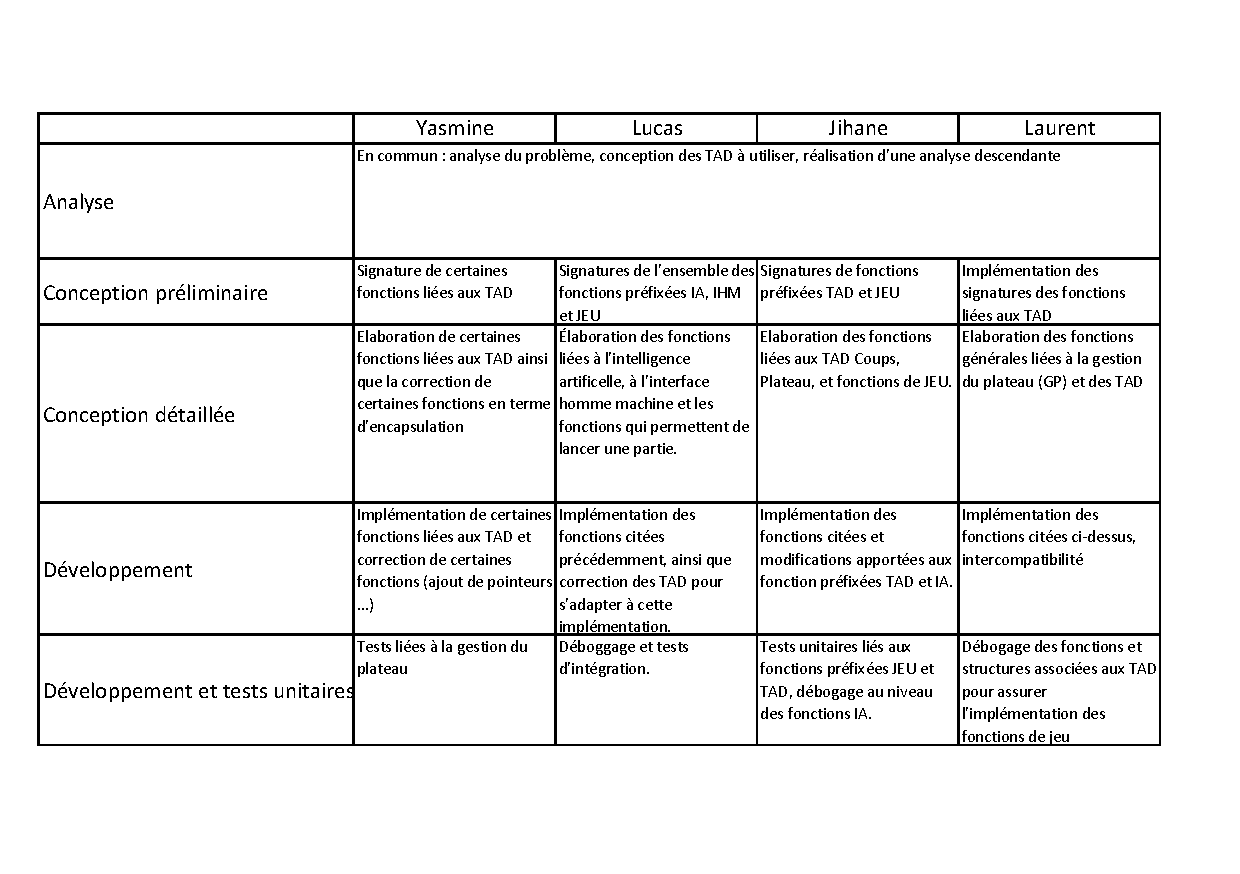
\includegraphics[scale=1, angle=0]{table_rep.pdf}}%
    \vspace*{\fill}

\end{document}
